\documentclass[12pt]{article}
\usepackage[paper=a4paper,left=25mm,right=25mm,top=30mm,bottom =30mm]{geometry}
\usepackage[utf8]{inputenc}
\usepackage[T1]{fontenc}
\usepackage{stmaryrd}
\usepackage{extarrows}
\usepackage{setspace}
\usepackage{mathrsfs}
\usepackage{mathtools}
\usepackage[ngerman]{babel}
\usepackage{amssymb}
\usepackage{amsmath}
\usepackage{fancyhdr}
\usepackage[dvips,unicode,colorlinks,linkcolor=black]{hyperref} 
\usepackage{graphicx}
\usepackage{float}




\pagestyle{fancy}
\lfoot{}
\rfoot{Paul Kremser, Tobias Grussenmeyer}
\cfoot{\thepage}
\fancyhead[L]{FPI Versuch: SQUID}
\renewcommand{\headrulewidth}{0.6pt}
\renewcommand{\footrulewidth}{0.6pt}
\setlength{\headheight}{16pt}
\setlength{\parindent}{0pt}
% Für die Wahl der Schriftart
\newcommand{\changefont}[3]{
\fontfamily{#1} \fontseries{#2} \fontshape{#3} \selectfont}

\begin{document}
% keine Hurenkinder und Schusterjungen
\clubpenalty = 10000
\widowpenalty = 10000 
\displaywidowpenalty = 10000

\onehalfspacing
% Schriftart
\changefont{ptm}{m}{n} 

\begin{titlepage}
\author{Paul Kremser, Tobias Grussenmeyer}
\title{Versuch: SQUID}
\date{Versuchsdurchführung: 22. Oktober 2009} 
\maketitle
\thispagestyle{empty}
\end{titlepage}


\tableofcontents
\thispagestyle{empty}
\newpage
\pagenumbering{arabic}
\section{Überblick}
In diesem Versuch soll mittels eines \textit{SQUID} das Magnetfeld verschiedener Proben sowie einer Stromdurchflossenen Leiterschleife gemessen und deren Dipolmoment bestimmt werden. Ein SQUID (\textbf{S}uper\-conducting \textbf{Qu}antum \textbf{I}nterference \textbf{D}evice) ist ein sehr kleiner, höchst empfindlicher Magnetfelddetektor, mit dem sich äußerst geringe Magnetfeldschwankungen registrieren lassen. Da die Nachweisgenauigkeit nur durch Quanteneffekte begrenzt ist, wird die Messgenauigkeit von keinem anderen Magnetfelddetektor übertroffen. Im wesentlichen besteht ein SQUID nur aus einem supraleitendem Ring der an einer sehr schmalen Stelle durch einen Isolator unterbrochen ist. Mit Hilfe geeigneter Elektronik können so kleinste Flussänderungen im Innern des Rings erkannt werden.


\section{Aufgabenstellung}
\begin{enumerate}
 \item Kalibration das SQUID durch Variation der Einstellungen. Es soll eine möglichst große Amplitude des SQUID-Patterns bei möglichst kleinem Rauschen gefunden werden.
\item Vermessung der Magnetfelder einer rotierender Leiterschleife welche von fünf verschiedenen Stromstärken durchflossen wird.  Bestimmung der Dipolmomente und Vergleich mit berechnetem Wert.
\item Vermessung der Magnetfelder und Dipolmomente verschiedener Proben (Magnetspan, Stabmagnet, Geldstück, SIM-Karte)
\item (optional) polare Darstellung der Stärke des Magnetfeldes in Abhängigkeit des Drehwinkels
\end{enumerate}
\newpage

\section{Theoretische Grundlagen}
\subsection{Supraleitung}
Bei der normalen elektrischen Leitung entsteht der elektrische Widerstand durch Wechselwirkungen der Elektronen mit Gitterfehlern des Kristallgitters und Gitterschwingungen. Darüber hinaus können auch Streuprozesse der Elektronen untereinander eine wichtige Rolle spielen. Vor der  Entdeckung der Supraleitung nahm man an, dass der elektrische Widerstand bei sinkender Temperatur asymptotisch gegen einen konstanten Wert (der nun nur noch aus der Wechselwirkung der Elektronen mit den Gitterfehlern resultiert) ginge. Anders als erwartet stellte sich jedoch heraus, dass für einige Stoffe der Wiederstand unterhalb einer kritischen Temperatur schlagartig einen nicht messbaren Wert annimmt. Dieses Phenomen bezeichnet man als Supraleitung. Unter Supraleitung versteht man also elektrische Leitung ohne messbaren Widerstand, man spricht auch von einem Suprastrom. \\
\begin{figure}[H]  %Gotische Kathedrale Kap. 4.1
\begin{minipage}{0.5\linewidth}
\centering
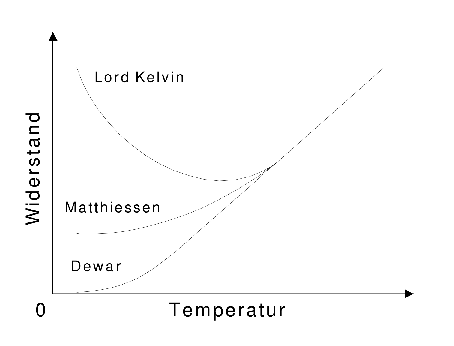
\includegraphics[width=0.9\linewidth]{pictures/wiederstandTemp.eps}
\caption{Elektrischen Widerstandes bei tiefen Temperaturen. Vorstellungen um 1900.}
\end{minipage}
\begin{minipage}{0.5\linewidth}
\centering 
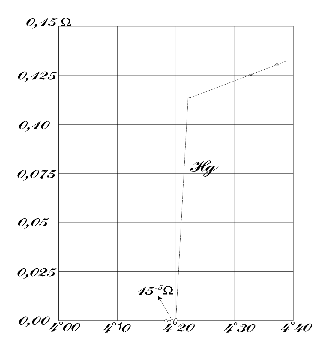
\includegraphics[width=0.9\linewidth]{pictures/HGJump.eps}
\caption{Sprungtemperatur von Quecksilber (Leiden 1911)}
\end{minipage}
\end{figure}

Allgemein wird die Supraleitung durch eine Paarbildung von Elektronen (Cooper-Paare) im Leiter erklärt(siehe hierzu \ref{bcs}).
 Durch die Kopplung der Elektronen im Supraleiter zu Cooper-Paaren wird die Energieabgabe an das Kristallgitter unterdrückt und so der widerstandslose elektrische Stromfluss ermöglicht. \\

Supraleiter sind ideale Diamagneten, im supraleitenden Zustand vermag ein Supraleiter bis zu einer oberen kritischen Grenze ein äußeres Magnetfeld (bis auf eine exponentiell abfallende Eindringtiefe an der Oberfläche, siehe \ref{london}) vollständig aus seinem Inneren zu verdrängen.\\

Es sind zwei Arten von Supraleitern bekannt: Typ-I und Typ-II.

Bei Typ I Supraleitern existiert nur eine obere kritische Grenze des äußeren Magnetfeldes. Unterhalb dieser befindet sich der Supraleiter in der Meißner-Phase, überschreitet das Magnetfeld diese Grenze so bricht die Supraleitung zusammen.\\

Bei Typ II Supraleitern gibt es zwei kritische äußere Magnetfelder, bis zum ersten kritischen Feld verhält sich der Supraleiter wie Typ I, darüber können magnetische Feldlinien in Form so genannter Flussschläuche in das Material eindringen, ehe der supraleitende Zustand bei dem oberen kritischen Magnetfeld vollständig zerstört wird. Der magnetische Fluss in den Flussschläuchen beträgt immer ein ganzzahliges Vielfaches des magnetischen Flussquants (siehe \ref{flussquantisierung}).\\

Bei unserem SQUID handelt es sich um einen Typ II Supraleiter. Beispiele für solche sind die keramischen Hochtemperatursupraleiter. Zwei wichtige Gruppen sind YBaCuO (Yttrium- Barium- Kupferoxide) und BiSrCaCuO (Bismut- Strontium- Kalzium- Kupferoxide). Weiterhin zählen die meisten supraleitenden Legierungen zum Typ II, so die für MR-Magnete verwendeten Niob-Aluminium-Legierungen.

\subsection{BCS-Theorie}
\label{bcs}
Nach der BCS-Thorie sind die Elektronen bei tiefer Temperatur gepaart. Die Kopplung beruht auf einer Wechselwirkung zwischen den Elektronen und dem Kristallgitter. Ein Elektron wechselwirkt mit dem Gitter und deformiert es. Das gestörte Gitter wechselwirkt, seinerseits mit einem anderen Elektron in der Weise, dass zwischen den beiden Elektronen eine Anziehung besteht, die bei niedrigen Temperaturen stärker als die Coulomb-Abstoßung ist. Die beiden Elektronen gehen in einen gebundenen Zustand über und bilden ein so genanntes Cooper-Paar. Die beiden Elektronen in einem Cooper-Paar haben entgegengesetzte Spins, so dass das Cooper-Paar als Ganzes den Spin null hat. Jedes Cooper-Paar verhält sich also wie ein Boson. Bosonen unterliegen nich dem Pauli-Verbot, so dass sich belibig viele Cooper-Paare im gleichen Quantenzustand befinden und die gleiche Energie besitzen können. Im Grundzustand des Supraleiters bei $T = 0K$ sind alle Elektronen in Cooper-Paaren gebunden, und alle Cooper-Paare haben dieselbe Energie. Im supraleitenden Zustand sind die Cooper-Paare stark korreliert und verhalten sich immer alle gleich. Der Stromfluss im Supraleiter wird dabei so realisiert, dass sich alle Elektronen in diesem Kollektiv gemeinsam bewegen. Dagegen kann Energiesissipation, die auf Stößen einzelner Elektronen mit den Gitterionen beruht, nicht stattfinden, es sei denn, die Temperatur ist so hoch, dass die Bindung der Cooper-Paare aufgebrochen wird.

\subsection{Flussquantisierung}
\label{flussquantisierung}

Bei einem SQUID handelt es sich um einen kreisförmigen Supraleiter, der Kreisstrom im Innern lässt sich also als Wegintegral über die Stromdichte $\vec{j}$ berechnen. Da dieser natürlich Null sein muss, folgt
\begin{align}
 \label{kreisstrom} \oint_C \vec j ~ d\vec l = 0
\end{align}

wobei $C$ der Weg entlang des SQUID's ist. Mit dem Stoke'schen Satz folgt das sich der magnetischen Fluss $\Phi_B$ durch den Ring darstellen lässt als das geschlossene Integral über das Vektorfeld $\vec A$:
\begin{align}
 \oint\vec A~d\vec l = \Phi_B
\end{align}

Die Cooper-Paare liegen wie oben beschrieben alle im gleichen Zustand vor, weshalb sie durch eine gemeinsame Wellenfunktion beschrieben werden können. Die Phase $\theta$ dieser Wellenfunktion ist ein eindeutiger Parameter, daher kann sie sich beim Umlauf um den Ring nur um Vielfache von $2\pi$ ändern:
\begin{align}
\label{phase}\oint \vec\nabla \theta d\vec l = \Delta\theta = n~2\pi
\end{align}

Aus Gleichungen \ref{kreisstrom} - \ref{phase} folgt somit eine Quantisierung des magnetischen Flusses in Vielfache von $\Phi_0$, Fluxoide genannt:
\begin{align}
  \left|\Phi_B\right| &= n\frac{\hbar c}{2 e} = n \Phi_0 \\
\notag \\
\notag \textnormal{mit}~~\Phi_0 &= 2,067833667(52)\cdot 10^{-15} ~ Wb \quad \quad (1[Wb] = 1[Tm^2])
\end{align}

\newpage

\subsection{London-Gleichungen}
\label{london}
Die Londongleichungen geben Aufschluss über die Eindringtiefe eines äußeren Magnetfelds in einen Supraleiter.
Hierzu wird angenommen, dass Beschleunigung von Ladungen $e$ nur von einem statischen elektrischen Feld $\vec E$ herrühren:
\begin{align}
 m~\dot{\vec{v}}_e = - e~ \vec E
\end{align}
Dies zusammen mit der Stromdichte $\vec j = n_e e~\vec v_e$, wobei $n_e$ Ladungsdichte, in die beiden Maxwellgleichungen:
\begin{align}
 \vec\nabla \times \vec E = - \frac{1}{c}\frac{\partial\vec B}{\partial t} \textnormal{\quad und \quad} 
 \vec\nabla \times \vec B =  \frac{4~\pi}{c}~\vec j
\end{align}
- durch ableiten der Stromdichte nach der Zeit - eingesetzt, liefert
\begin{align}
 \frac{\partial}{\partial t} \left( \vec\nabla\times\vec j +  \frac{n_e~e^2}{m~c}~\vec B\right) = 0
\end{align}
Dies fordert Zeitliche Invarianz des Ausdrucks in der Klammer, da $\vec B$ im inneren des Supraleiters aber Null ist, folgt dass die Klammer Null sein muss. Somit kommt man auf die London-Gleichung:
\begin{align}
 \vec\nabla\times\vec j = -\frac{n_e~e^2}{m~c}~\vec B
\end{align}
aus der sich die beiden Gleichungen:
\begin{align}
 \nabla^2~\vec B = \frac{4~\pi~n_e~e^2}{m~c^2}~\vec B \textnormal{\quad und \quad} \nabla^2~\vec j = \frac{4~\pi~n_e~e^2}{m~c^2}~\vec j
\end{align}
ableiten lassen. Lösungen für diese sind exponentiell abfallende Funktionen mit einer Reichweite von $\Lambda =\sqrt{\frac{m~c^2}{4~\pi~n_e~e^2}}$. Folglich kann ein äußeres Magnetfeld eine gewisse Länge in einen Supraleiter eindringen. In der vom Magnetfeld durchdrungenen Schicht fließt außerdem ein Abschirmstrom senkrecht zum Magnetfeld.

\subsection{Josephson-Effekt}
\label{josephson}

Der Josephson-Effekt besagt, dass Cooper-Paare widerstandsfrei zwischen zwei Supraleitern tunneln, die durch eine dünne, nichtsupraleitende Schicht voneinander getrennt sind. Eine solche Anordnung nennt man \textbf{Josephson-Kontakt}. Der Tunnelstrom tritt auf, ohne dass eine Spannung über dem Kontakt angelegt wird. Der Strom hängt von der Phasendifferenz der Wellenfunktion der Cooper-Paare in den beiden Supraleitern ab. Sei $\phi_1$ die Phase der Wellenfunktion eines Cooper-Paars in dem einen Supraleiter. Dann haben auch alle anderen Cooper-Paare in diesem Supraleiter die Phase $\phi_1$, da sich alle Cooper-Paare in einem Supraleiter kohärent verhalten. Ist $\phi_2$ die Phase der Wellenfunktionen aller Cooper-Paare im zweiten Supraleiter, so beträgt der Strom durch die Übergangsschicht:
\begin{align}
\label{jos-gleichstrom}
 I = I_{max}~sin(\phi_2 - \phi_1)
\end{align}
Darin ist $I_{max}$ der maximale Strom. Dieser ist von der Dicke der Kontaktschicht abhängig. Die Gleichung \ref{jos-gleichstrom} beschreibt die Abhängigkeit die als \textbf{Josephson-Gleichstrom-Effekt} bezeichnet wird.

\subsection{Das SQUID}

Das SQUID kann also kleinste magnetische Flussänderungen in der grössenordnung eines Flussquants registrieren. Es gibt verschiedene technische Umsetzungen, hier im Praktikum  nutzen wir ein sogenanntes RF-SQUID(RF = Radio Frequency),  ein vergleichsweise einfacher und günstiger Aufbau.

\subsection{Aufbau des RF-SQUID}
\subsection{Arbeitspunkt des SQUIDs}

\subsection{Lock-In Verstärker}

\section{Versuchsaufbau}

\section{Durchführung}

\section{Auswertung}

\section{Zusammenfassung}



\end{document}
